% Provenance (never printed): see sources/outline_sources.md (Year 2: palaeogeography through
% the Phanerozoic; sea level; orogenies; mass extinctions and their Earth causes). Maps from the
% plate model of Merdith and others (2021) through the GPlates Web Service; sea level from the
% Miller and others (2005) NOAA study (Haq and others 1987; Kominz and others 2008); flooding and
% the Pitman model after Tasistro-Hart and Macdonald (2023); the big five after Marshall (2023)
% and Kaiho (2022); oceanic anoxic events after Rigo and others (2024) and Walker-Trivett and
% others (2024); CAMP carbon dioxide after Capriolo and others (2020); Chicxulub after
% Pickersgill and others (2026) and Collins and others (2020). Curves and numbers from
% figdata/bachelor-2/phanerozoic.py; exercise and problem values in the Book 4 scratch
% calculator calc/ch19.py.
\chapter{फ़ैनेरोज़ोइक पृथ्वी}\label{ch:b2:phanerozoic-earth}

पश्चिमी कैनसस में, उत्तर अमेरिका के बीचोबीच, सफ़ेद खड़िया के स्तंभ घास के मैदान से उठते हैं।
यह खड़िया एक समुद्र-तल का ऊज़ है: लगभग 80 मिलियन वर्ष पहले एक
उथला समुद्र उत्तर अमेरिका के बीच से उत्तर से दक्षिण तक फैला था, और तैरते शैवालों के कवच
उसके तल पर वर्ष में मिलीमीटर के कुछ सौवें भाग की दर से बैठते थे। पिछले 540 मिलियन वर्षों में पाँच बार,
ऐसे समुद्रों में रहने वाली प्रजातियों का एक बड़ा भाग एक भूवैज्ञानिक क्षण में लुप्त हो गया।
दोनों कहानियाँ पृथ्वी की अपनी हैं: महाद्वीप खिसके और समुद्र उन पर चढ़ा और उतरा,
और पाँच महान विलोपनों में से कम से कम तीन ग्रह के भीतर से उमड़े लावा के साथ घटे।
यह अध्याय फ़ैनेरोज़ोइक को उसके मानचित्रों, उसके समुद्र-स्तर, उसकी पर्वत-पट्टियों
और उसके संकटों के सहारे देखता है, और उनमें से दो को संख्याएँ देता है: कटक समुद्र को कितनी तेज़ी से उठाते हैं, और
ऊँचा समुद्र कितनी भूमि डुबो देता है।
% ledger: kgs:monument-rocks, kgs:chalk, ics:base.Phanerozoic, kaiho22:table, cr03:table

\begin{recall}
\textbf{स्कूल की पुस्तकों से}: प्लेट विवर्तनिकी और पैंजिया; जीवाश्म और भूवैज्ञानिक समय-मापक्रम;
किसी खड़ी चट्टान में पढ़े गए ट्रांसग्रेशन। \textbf{पुस्तक 3 (स्नातक वर्ष 1) से}: महासागर-तल का गहराई--आयु
नियम; हिप्सोमेट्रिक वक्र; समस्थिति; यूस्टेसी और सापेक्ष समुद्र-स्तर; बृहत आग्नेय
प्रांत; कालस्तरिक चिह्नकों के रूप में सामूहिक विलोपन, K--Pg सीमा का इरिडियम और
पर्मियन-अंत संकट का काल-निर्धारण; चरण और GSSP। \textbf{पिछले अध्यायों से}: \omterm{def:b2:alpine-orogen:orogen}{पर्वतजनक पट्टियाँ}
(\cref{ch:b2:alpine-orogen,ch:b2:himalaya-andes}); \omterm{def:b2:wilson-cycle:wilson}{विल्सन चक्र} और \omterm{def:b2:wilson-cycle:supercontinent}{महामहाद्वीप}
(\cref{ch:b2:wilson-cycle}); \omterm{def:b2:basins-compared:backstripping}{बैकस्ट्रिपिंग} (\cref{ch:b2:basins-compared}); क्रायोजेनियन के
हिमगोल (\cref{ch:b2:precambrian-earth})। विलोपन और जीवन का इतिहास जीवविज्ञान की पुस्तकों
के विषय हैं; पुराचुंबकत्व और अनुक्रम स्तरिकी का विवेचन पुस्तक 5 करती है।
\end{recall}

\section{एक गतिशील संसार के मानचित्र}\label{sec:b2:phanerozoic-earth:maps}

कोई चट्टान शायद ही वहाँ होती है जहाँ वह बनी थी। कोयला, मरुस्थली बलुआ पत्थर, प्रवाल-भित्ति: हर एक किसी
अक्षांश पर बिछा था और तब से अपनी प्लेट के साथ ढोया गया है। ऐसी चट्टानों से किसी बीते समय की
जलवायु या जीवन पढ़ने से पहले उन्हें वहीं वापस रखना होता है जहाँ वे थीं।

\begin{definition}[पुराभूगोल; पुराभौगोलिक मानचित्र]\label{def:b2:phanerozoic-earth:palaeogeography}
\emph{पुराभूगोल}\index{पुराभूगोल} किसी बीते समय के भूगोल का पुनर्निर्माण है:
महाद्वीपों और महासागरों की स्थितियाँ, और उनकी तट-रेखाओं, पर्वत-पट्टियों और
समुद्रों की। एक \emph{पुराभौगोलिक मानचित्र}\index{पुराभौगोलिक मानचित्र} उस भूगोल को एक
समय पर, उसी समय के अक्षांश और देशांतर के जाल पर, दिखाता है।
\end{definition}

ऐसे मानचित्र में चार प्रकार के साक्ष्य जाते हैं। चट्टानों का चुंबकन वह अक्षांश देता है जिस पर
वे बनीं, जो पुस्तक 5 में पुराचुंबकत्व का विषय है; पर पृथ्वी का क्षेत्र अपनी अक्ष के प्रति
सममित है, इसलिए वह देशांतर के बारे में कुछ नहीं कहता। महासागर-तल अपनी चुंबकीय पट्टियों और अपनी आयुओं से
प्लेटों की गति को सीधे दर्ज करता है, पर केवल
बचे हुए सबसे पुराने तल तक, लगभग 190 मिलियन वर्ष: उससे पुराना सब कुछ क्षेपित हो चुका है। उससे पहले,
महाद्वीपों का मेल, वे सीवनें और \omterm{def:b2:alpine-orogen:orogen}{पर्वतजनक पट्टियाँ} जहाँ महासागर बंद हुए, और वे जीवाश्म और
अवसाद जो किसी जलवायु को प्रकट करते हैं --- उष्णकटिबंध में प्रवाल-भित्तियाँ और वाष्पनिक निक्षेप, ध्रुवों के पास हिमनदीय
निक्षेप --- चित्र पूरा करते हैं। प्लेट मॉडल इन बाधाओं को इकट्ठा करते हैं और हर प्लेट को समय में
पीछे घुमाते हैं; पुनर्निर्माणों को पूरी ठोस पृथ्वी के उसकी घूर्णन-अक्ष के सापेक्ष धीमे घूर्णन का भी
ध्यान रखना पड़ता है, जिसे सच्चा ध्रुवीय भ्रमण कहते हैं।
% ledger: vh26:palaeogeography, gws:merdith-frame, data:b2-seafloor-age, merdith21:model

\begin{omfigure}
\centering
% figdata/bachelor-2/phanerozoic.py parts map-<t>, cities-<t>, grat (Mollweide, x and y in Earth radii)
\begin{tikzpicture}
\begin{groupplot}[group style={group size=2 by 3, horizontal sep=0.35cm, vertical sep=0.55cm},
  width=0.53\linewidth, axis equal image, hide axis, clip=false,
  xmin=-2.85, xmax=2.85, ymin=-1.43, ymax=1.43,
  title style={font=\small, yshift=-1.5ex}]
\pgfplotsinvokeforeach{500,300,200,100,50,0}{
\nextgroupplot[title={#1~\unit{Ma}}]
\fill[omSea] (axis cs:0,0) ellipse [x radius=2.8284, y radius=1.4142];
\addplot[fill=omLithAlluv!85!black, draw=none] table[x=x, y=y]
  {figdata/out/bachelor-2-phanerozoic-map-#1.dat};
\addplot[black!35, line width=0.2pt] table[x=x, y=y] {figdata/out/bachelor-2-phanerozoic-grat.dat};
\draw[black!70, line width=0.4pt] (axis cs:0,0) ellipse [x radius=2.8284, y radius=1.4142];
\addplot[only marks, mark=*, mark size=1.3pt, red!75!black, point meta=explicit symbolic,
  nodes near coords, nodes near coords style={font=\tiny\bfseries, anchor=south west,
  inner sep=0.5pt, text=red!60!black}]
  table[x=x, y=y, meta=tag] {figdata/out/bachelor-2-phanerozoic-cities-#1.dat};
}
\end{groupplot}
\end{tikzpicture}
\par\smallskip{\small आज की तट-रेखाएँ मर्डिथ और अन्य (2021) के प्लेट मॉडल में छह समयों तक
पीछे ले जाई गईं, जीप्लेट्स वेब सेवा द्वारा पुनर्निर्मित, एक समक्षेत्र मॉलवाइड
प्रक्षेप में; अक्षांश-रेखाएँ हर \ang{30} पर, देशांतर-रेखाएँ हर \ang{60} पर। लाल बिंदु चार
नगरों का अनुसरण करते हैं: पेरिस (P), न्यूयॉर्क (N), सिडनी (S) और केप टाउन (C); \qty{500}{Ma} पर
सिडनी की भूपर्पटी अभी मॉडल में नहीं है। आकृतियाँ आज की तट-रेखाएँ हैं जिन्हें खिसकाया गया है, उन
समयों की तट-रेखाएँ नहीं, और इस पुराचुंबकीय ढाँचे में देशांतर मनमाने हैं।}
\end{omfigure}
% ledger: data:b4-palaeocoast, data:b4-palaeopos, geonames4:cities, gws:merdith-frame, merdith21:model

ऊपर के छह मानचित्र संक्षेप में फ़ैनेरोज़ोइक हैं। \qty{500}{Ma} पर दक्षिणी महाद्वीप
एक पिंड बनाते हैं, गोंडवाना, जिसका बड़ा भाग दक्षिणी ध्रुव के पास है, और पेरिस की भूपर्पटी \ang{61}~S पर उसके
किनारे पर है। \qty{300}{Ma} तक महाद्वीप जुड़कर पैंजिया बन चुके हैं, जो लगभग
\qty{325}{Ma} से जुड़ा और लगभग \qty{200}{Ma} से टूटा: पेरिस और न्यूयॉर्क भूमध्य रेखा पर हैं, केप
टाउन और सिडनी \ang{60}~S के पास। \qty{200}{Ma} पर \omterm{def:b2:wilson-cycle:supercontinent}{महामहाद्वीप} पूरा है, एक अकेली भूमि
जो उच्च उत्तरी से उच्च दक्षिणी अक्षांशों तक फैली है; \qty{100}{Ma} तक अटलांटिक और हिंद महासागर खुल चुके हैं, और
\qty{50}{Ma} तक मानचित्र लगभग आज का है, ऑस्ट्रेलिया अभी भी अंटार्कटिका के पास।
% ledger: data:b4-palaeopos, nance22:supercontinents

\begin{example}[पेरिस उत्तर की ओर खिसकता है]\label{ex:b2:phanerozoic-earth:paris}
मॉडल में पेरिस \ang{5.1}~N पर \qty{300}{Ma} पहले था; आज वह \ang{48.9}~N पर है। उसका
अक्षांश \ang{43.8} बढ़ा है, यानी एक याम्योत्तर के अनुदिश $43.8 \times 111.2 = \qty{4871}{km}$
($\qty{111.2}{km}$ प्रति अंश, \qty{6371}{km} त्रिज्या के गोले पर), औसत दर
$4871/300 = \qty{16}{km}$ प्रति मिलियन वर्ष, या \qty{1.6}{cm} प्रति वर्ष। यह गति का केवल उत्तरमुखी
भाग है: पुराचुंबकीय ढाँचा देशांतर को मुक्त छोड़ता है, इसलिए वास्तव में तय की गई
दूरी कम से कम इतनी थी।
\end{example}
% ledger: data:b4-palaeopos, geonames4:cities, earth:Rmean, gws:merdith-frame
% values: calc/ch19.py (43.8 deg, 4870.6 km, 16.2 km/Myr)

\section{फ़ैनेरोज़ोइक में समुद्र-स्तर}\label{sec:b2:phanerozoic-earth:sealevel}

\subsection*{महाद्वीपों पर समुद्र}

फ़ैनेरोज़ोइक के अधिकांश समय में महाद्वीपों का कहीं अधिक भाग आज की तुलना में समुद्र के नीचे था।
उत्तर अमेरिका की समुद्री चट्टानें महाद्वीप के भीतरी भाग की कई बाढ़ों को दर्ज करती हैं, उनमें
पहली कैम्ब्रियन ट्रांसग्रेशन है जो महा विषमविन्यास को ढकती है; उत्तर क्रिटेशियस में,
लगभग 120 से \qty{80}{Ma} तक, समुद्री अवसाद पश्चिमी आंतरिक भाग में, महाद्वीप के
बीच में, जमा हुए (नीचे का फ़ोटो)।
% ledger: th23:flooding, th23:wib

\begin{omfigure}
\centering
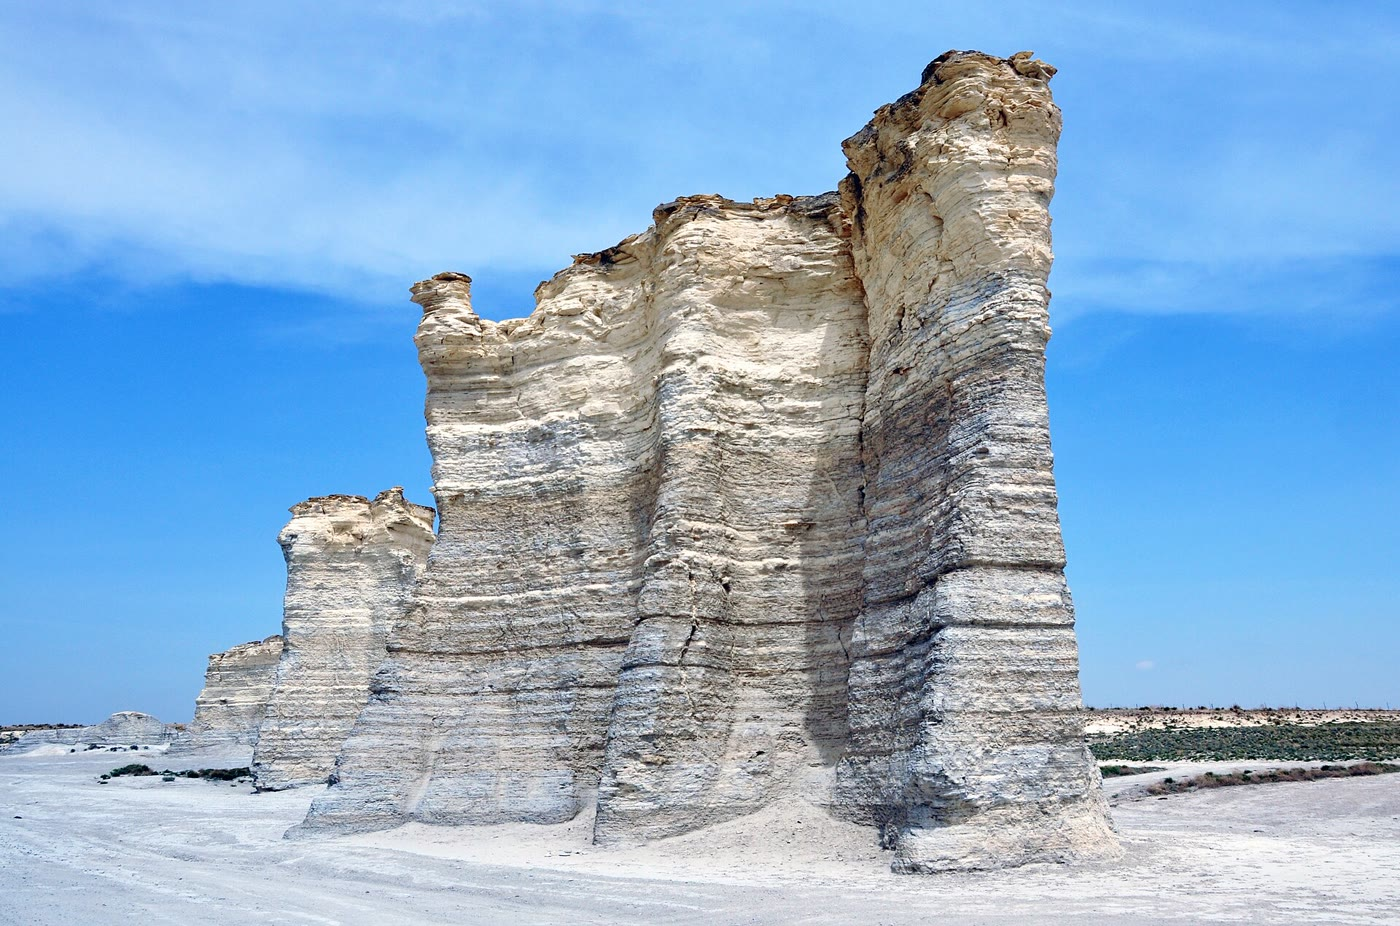
\includegraphics[width=0.66\linewidth]{images/book4/b2-19-monument-rocks.jpg}
\par\smallskip{\small मॉन्यूमेंट रॉक्स, पश्चिमी कैनसस: खड़िया के स्तंभ, एक क्रिटेशियस
अंतर्देशीय समुद्र का लगभग 80 मिलियन वर्ष पुराना ऊज़, जो लगभग \qty{0.036}{mm} प्रति वर्ष की दर से जमा। (James
St.~John, CC~BY~2.0, विकिमीडिया कॉमन्स के माध्यम से।)}
\end{omfigure}
% ledger: kgs:monument-rocks, kgs:chalk

\begin{definition}[अधिमहाद्वीपीय सागर]\label{def:b2:phanerozoic-earth:epeiric}
एक \emph{अधिमहाद्वीपीय सागर}\index{अधिमहाद्वीपीय सागर} किसी महाद्वीप के भीतरी भाग पर फैला एक उथला समुद्र है,
महाद्वीपीय भूपर्पटी पर, महाद्वीपीय किनारे से दूर।
\end{definition}

समुद्र अपना तट खिसकाकर ऐसे भीतरी भागों तक पहुँचता है, और चट्टानें उस गति को दर्ज करती हैं।

\begin{definition}[समुद्री ट्रांसग्रेशन; समुद्री रिग्रेशन]\label{def:b2:phanerozoic-earth:transgression}
\emph{समुद्री ट्रांसग्रेशन}\index{समुद्री ट्रांसग्रेशन} (अतिक्रमण) तट-रेखा का भूमि की ओर खिसकना है,
जिससे समुद्र भूमि पर फैलता है; \emph{समुद्री रिग्रेशन}\index{समुद्री रिग्रेशन} (अपगमन)
समुद्र की ओर खिसकना है, जिससे भूमि बाहर निकल आती है।
\end{definition}

एक ऊर्ध्वाधर खंड में ट्रांसग्रेशन गहरे जल के निक्षेपों को उथले निक्षेपों पर रखता है ---
तट से दूर की कीचड़ समुद्र-तट की बालू पर --- और रिग्रेशन इसका उलटा। दोनों सापेक्ष समुद्र-स्तर
का अनुसरण करते हैं, जो वैश्विक समुद्र-स्तर को स्थान के अवधसान या उत्थान से और
अवसाद की आपूर्ति से मिलाता है: समुद्र उठते समय भी एक डेल्टा अपना तट समुद्र की ओर धकेल सकता है, यदि उसे पर्याप्त
तेज़ी से पोषण मिले। ट्रांसग्रेशनों से वैश्विक समुद्र-स्तर पढ़ने के लिए भूविज्ञानी को वही संकेत
कई महाद्वीपों पर खोजना होगा, या \omterm{def:b2:basins-compared:backstripping}{बैकस्ट्रिपिंग} से अवधसान को हटाना होगा, जैसा
\cref{ch:b2:basins-compared} में।
% ledger: miller20:rsl

\subsection*{दीर्घकालिक वक्र}

\begin{definition}[प्रथम-कोटि समुद्र-स्तर चक्र]\label{def:b2:phanerozoic-earth:first-order}
\emph{प्रथम-कोटि समुद्र-स्तर चक्र}\index{प्रथम-कोटि समुद्र-स्तर चक्र} वैश्विक समुद्र-स्तर के परिवर्तन का सबसे धीमा
भाग है, दसियों से सैकड़ों मिलियन वर्षों के समय-पैमानों पर, जिसे हिम नहीं बल्कि
ठोस पृथ्वी की विवर्तनिकी तय करती है।
\end{definition}

पूरे फ़ैनेरोज़ोइक में प्रथम-कोटि वक्र का आकार M जैसा है: आरंभिक पैलियोज़ोइक में ऊँचा,
जब पैंजिया जुड़ा और टिका रहा, कार्बोनिफ़ेरस से ट्राइऐसिक के अंत तक, तब नीचा, क्रिटेशियस में फिर
ऊँचा, और तब से गिरता हुआ। उत्तर अमेरिका से बहिर्वेशन करने पर, अकेली उत्तर
ऑर्डोविशियन बाढ़ 100 से \qty{200}{m} की और वृद्धि सुझाती है।
इस वक्र पर तेज़ परिवर्तन सवार हैं: हिम से चलने वाले परिवर्तन $10^4$ से
$10^6$ वर्षों के समय-पैमानों पर दर्ज हैं, और अंटार्कटिक हिमचादर ने, लगभग \qty{33.5}{Ma} से, समुद्र को 50 से
\qty{60}{m} खिसकाया।
% ledger: th23:flooding, miller11:greenhouse, miller05:abstract

\begin{omfigure}
\centering
% figdata/bachelor-2/phanerozoic.py parts sealevel-haq, sealevel-haqlt, sealevel-kominz, sealevel-kominzlt
\begin{tikzpicture}
\begin{axis}[width=0.92\linewidth, height=6.2cm, x dir=reverse, xmin=0, xmax=252,
  ymin=-130, ymax=280, xlabel={आयु (\unit{Ma})}, ylabel={आज से ऊपर समुद्र-स्तर (\unit{m})},
  xtick={0,50,...,250}, ytick={-100,-50,...,250}, xtick pos=bottom, ytick pos=left,
  tick label style={font=\scriptsize}, label style={font=\small},
  legend style={at={(0.5,1.04)}, anchor=south, draw=none, font=\scriptsize, legend columns=2,
  /tikz/every even column/.append style={column sep=8pt}}]
\addplot[black!30, line width=0.3pt] table[x=age_ma, y=sl_m]
  {figdata/out/bachelor-2-phanerozoic-sealevel-haq.dat};
\addlegendentry{हक़ और अन्य (1987)}
\addplot[omThm, line width=0.3pt] table[x=age_ma, y=sl_m]
  {figdata/out/bachelor-2-phanerozoic-sealevel-kominz.dat};
\addlegendentry{न्यू जर्सी, बैकस्ट्रिप किया}
\addplot[black, line width=1.2pt] table[x=age_ma, y=sl_m]
  {figdata/out/bachelor-2-phanerozoic-sealevel-haqlt.dat};
\addlegendentry{हक़, 10 मिलियन वर्ष का माध्य}
\addplot[omThm!70!black, line width=1.2pt] table[x=age_ma, y=sl_m]
  {figdata/out/bachelor-2-phanerozoic-sealevel-kominzlt.dat};
\addlegendentry{न्यू जर्सी, 10 मिलियन वर्ष का माध्य}
\addplot[black!50, line width=0.3pt, forget plot] coordinates {(0,0) (252,0)};
\foreach \a/\b/\c in {251.902/201.4/icsTriassic, 201.4/143.1/icsJurassic,
  143.1/66/icsCretaceous, 66/23.04/icsPaleogene, 23.04/2.58/icsNeogene, 2.58/0/icsQuaternary} {
  \edef\tmp{\noexpand\fill[\c] (axis cs:\a,-130) rectangle (axis cs:\b,-112);}\tmp}
\node[font=\tiny, text=white] at (axis cs:226.7,-121) {ट्राइऐसिक};
\node[font=\tiny, text=white] at (axis cs:172.3,-121) {जुरैसिक};
\node[font=\tiny] at (axis cs:104.6,-121) {क्रिटेशियस};
\node[font=\tiny] at (axis cs:44.5,-121) {पैलियोजीन};
\node[font=\tiny] at (axis cs:12.8,-121) {नियो॰};
\end{axis}
\end{tikzpicture}
\par\smallskip{\small \qty{250}{Ma} से वैश्विक समुद्र-स्तर, जैसा मिलर और अन्य
(2005) ने सारणीबद्ध किया: हक़ और अन्य (1987) का चक्र-चार्ट, अनेक द्रोणियों की स्तरिकी से, और
न्यू जर्सी के कोर-छिद्रों से बैकस्ट्रिप किया गया समुद्र-स्तर, अनुमानित निम्नतम स्तरों के साथ (कोमिंज़ और
अन्य 2008)। मोटी रेखाएँ: 10 मिलियन वर्ष के चल माध्य, प्रथम-कोटि प्रवृत्ति। आयु 2012 के समय-मापक्रम
पर; नीचे की पट्टी कालों को दिखाती है।}
\end{omfigure}
% ledger: data:b4-sealevel, haq87:charts, kominz08:long-term, ics:base.Triassic, ics:base.Jurassic, ics:base.Cretaceous, ics:base.Paleogene, ics:base.Neogene, ics:base.Quaternary, ics:colour.Triassic, ics:colour.Jurassic, ics:colour.Cretaceous, ics:colour.Paleogene, ics:colour.Neogene, ics:colour.Quaternary

ऊपर के दो वक्र आकार पर सहमत हैं और परिमाण पर असहमत। चक्र-चार्ट, जो अनेक द्रोणियों में
अवसादों के जमाव से बना है, मध्य-क्रिटेशियस के दीर्घकालिक समुद्र-स्तर को आज के स्तर से
लगभग \qty{233}{m} ऊपर रखता है; न्यू जर्सी के कुएँ, एक-एक कर बैकस्ट्रिप किए गए, उत्तर क्रिटेशियस में लगभग
\qty{70}{m} और इओसीन में लगभग \qty{110}{m} का अधिकतम देते हैं। मिलर और उनके
सहयोगी निष्कर्ष निकालते हैं कि क्रिटेशियस का दीर्घकालिक शिखर $100 \pm \qty{50}{m}$ था, और कि
चक्र-चार्ट, गिरावटों के समय के बारे में सही होते हुए भी, उनके आयामों को बढ़ा-चढ़ाकर दिखाते हैं। न्यू जर्सी भी
पूर्ण मापक नहीं है: उसका उत्तर क्रिटेशियस समुद्र उस स्तर से 100 से \qty{150}{m} नीचा है जो
महासागर द्रोणियों का आयतन बताता है, एक अंतर जिसे क्षेपित फ़ैरालॉन प्लेट के ऊपर
क्षेत्र का धँसना --- गतिक स्थलाकृति --- समझा सकता है।
% ledger: data:b4-sealevel, miller05:abstract, kominz08:long-term, miller20:epr

\subsection*{समुद्र क्यों खिसकता है: कटक}

दसियों मिलियन वर्षों तक समुद्र को सौ मीटर ऊपर क्या रखता है? हिम नहीं: क्रिटेशियस
एक गर्म संसार था, जिसमें अधिक से अधिक छोटी, अल्पजीवी हिमचादरें थीं। प्रमुख उत्तर
महासागरीय कटकों का आयतन है। युवा महासागर-तल गर्म होता है और ऊँचा खड़ा रहता है; प्लेटें जितनी तेज़ी से फैलती हैं,
तल औसतन उतना ही युवा, महासागर द्रोणियाँ उतनी ही उथली, और उतना ही अधिक जल
महाद्वीपों पर फैलता है।
% ledger: miller11:greenhouse, th23:pitman

\begin{proposition}[समुद्र-स्तर और प्रसरण-दर]\label{prop:b2:phanerozoic-earth:ridge}
मान लीजिए क्षेत्रफल $A_{\text{f}}$ का महासागर-तल कुल लंबाई $L$ के कटकों पर पूर्ण
प्रसरण-दर $u$ से बनता है, और आयु $\tau = A_{\text{f}}/(Lu)$ पर नष्ट होता है, 0
और $\tau$ के बीच की हर आयु समान क्षेत्रफल घेरती है। उसकी गहराई नियम $d(t) = d_{\text{r}} + c\sqrt t$ का पालन करे।
\begin{enumerate}
  \item तल की माध्य गहराई $\bar d = d_{\text{r}} + \tfrac23 c\sqrt\tau$ है।
  \item यदि प्रसरण-दर $fu$ हो जाए, $A_{\text{f}}$ और $L$ अपरिवर्तित रहें, तो माध्य
        गहराई $\Delta\bar d = \tfrac23 c\sqrt\tau\,\bigl(1 - f^{-1/2}\bigr)$ घटती है।
  \item यदि तल जोड़े गए जल के नीचे समस्थैतिक रूप से धँसे, और समुद्र भूमि पर न
        फैले, तो क्षेत्रफल $A_{\text{o}}$ के महासागर पर समुद्र-स्तर इतना उठता है:
        \[
        \Delta s = \frac{\rho_{\text{m}} - \rho_{\text{w}}}{\rho_{\text{m}}}\,
        \frac{A_{\text{f}}}{A_{\text{o}}}\,\Delta\bar d ,
        \]
        जहाँ $\rho_{\text{m}}$ प्रावार का घनत्व है और $\rho_{\text{w}}$ समुद्री जल का।
\end{enumerate}
\end{proposition}

\begin{proof}
(1) कटक नया तल $Lu$ (प्रति इकाई समय क्षेत्रफल) की दर से बनाते हैं, और तल की हर पट्टी
समय $\tau$ तक जीती है; स्थायी अवस्था में $t$ और $t + \mathrm{d}t$ के बीच आयु वाले तल का क्षेत्रफल
$Lu\,\mathrm{d}t$ है, हर $t < \tau$ के लिए, इसलिए कुल क्षेत्रफल $Lu\tau = A_{\text{f}}$ है और
आयुएँ समान रूप से फैली हैं। माध्य गहराई है
$\frac1\tau\int_0^\tau (d_{\text{r}} + c\sqrt t)\,\mathrm{d}t = d_{\text{r}} + \frac{c}{\tau}
\cdot\frac23\tau^{3/2}$। (2) दर $fu$ के साथ $\tau$ बन जाता है $\tau/f$, और
$\sqrt{\tau/f} = f^{-1/2}\sqrt\tau$। (3) द्रोणियाँ आयतन $\Delta V = A_{\text{f}}
\Delta\bar d$ खोती हैं। मान लीजिए समुद्र-सतह महाद्वीपों के सापेक्ष $\Delta s$ उठती है, और तल
अतिरिक्त जल के नीचे $y$ धँसता है। अतिरिक्त जल-स्तंभ, $\Delta s + y$ मोटा, समस्थैतिक संतुलन में
प्रावार की $y$ मोटाई का स्थान लेता है: $\rho_{\text{w}}(\Delta s + y) =
\rho_{\text{m}} y$, इसलिए $y = \rho_{\text{w}}\Delta s/(\rho_{\text{m}} - \rho_{\text{w}})$ और
$\Delta s + y = \Delta s\,\rho_{\text{m}}/(\rho_{\text{m}} - \rho_{\text{w}})$। आयतन
संरक्षित है: $A_{\text{o}}(\Delta s + y) = \Delta V$, जिससे परिणाम मिलता है।
\end{proof}

वास्तविक तल इतना सुव्यवस्थित नहीं है। उसकी आयुएँ समान रूप से नहीं फैलीं: युवा तल सबसे अधिक है,
और आयु के साथ क्षेत्रफल घटता है, जैसा नीचे का बायाँ पैनल दिखाता है। न ही वर्गमूल नियम
पुराने तल पर लागू होता है, जो लगभग \qty{6.4}{km} के पास चपटा हो जाता है; पार्सन्स और स्क्लेटर ने पुराने तल पर
जो चरघातांकी नियम बिठाया, प्लेट नियम, वह लगभग \qty{26}{Myr} के बाद स्थान लेता है, जहाँ दोनों नियम
मिलते हैं। प्रस्ताव एक पहला अनुमान है, और चित्र
दिखाता है कि दूसरा नियम उसे कितना बदलता है।
% ledger: ps77:depth-age, data:b4-ridge

\begin{omfigure}
\centering
% figdata/bachelor-2/phanerozoic.py parts agehist and ridge
\begin{tikzpicture}
\begin{groupplot}[group style={group size=2 by 1, horizontal sep=1.6cm},
  width=0.5\linewidth, height=5.6cm, tick label style={font=\scriptsize},
  label style={font=\small}, xtick pos=bottom, ytick pos=left]
\nextgroupplot[xmin=0, xmax=200, ymin=0, ymax=34, xlabel={तल की आयु (\unit{Myr})},
  ylabel={प्रति \qty{10}{Myr} क्षेत्रफल (\unit{\mega km^2})},
  legend style={at={(0.5,1.04)}, anchor=south, draw=none, font=\scriptsize}]
\addplot[ybar interval, area legend, fill=omSea!80!black, draw=black!50, line width=0.2pt]
  table[x expr=\thisrow{age}-5, y=area_Mkm2] {figdata/out/bachelor-2-phanerozoic-agehist.dat};
\addlegendentry{आयु-ग्रिड}
\addplot[const plot mark mid, black, dashed, line width=0.9pt]
  table[x=age, y=uniform_Mkm2] {figdata/out/bachelor-2-phanerozoic-agehist.dat};
\addlegendentry{\qty{128.4}{Myr} तक समान आयुएँ}
\nextgroupplot[xmin=1, xmax=3, ymin=0, ymax=650, xlabel={प्रसरण-दर / आज की, $f$},
  ylabel={समुद्र-स्तर वृद्धि $\Delta s$ (\unit{m})},
  legend style={at={(0.5,1.04)}, anchor=south, draw=none, font=\scriptsize, legend columns=2}]
\fill[omThm!15] (axis cs:1,50) rectangle (axis cs:3,150);
\addplot[black, line width=1pt] table[x=f, y=ds_hs] {figdata/out/bachelor-2-phanerozoic-ridge.dat};
\addlegendentry{$\sqrt t$ नियम}
\addplot[blue!70!black, dashed, line width=1pt] table[x=f, y=ds_plate]
  {figdata/out/bachelor-2-phanerozoic-ridge.dat};
\addlegendentry{प्लेट नियम}
\node[font=\scriptsize, anchor=west] at (axis cs:1.6,100) {$100 \pm \qty{50}{m}$};
\end{groupplot}
\end{tikzpicture}
\par\smallskip{\small बायाँ: आज के महासागर-तल का 10 मिलियन वर्ष के आयु-खंडों में क्षेत्रफल, सेटन और अन्य (2020) के
एक-अंश विभेदन वाले आयु-ग्रिड से (कुल \qty{293}{\mega km^2}), उसी क्षेत्रफल और माध्य आयु वाले
\cref{prop:b2:phanerozoic-earth:ridge} के समान फैलाव की तुलना में। दायाँ:
प्रसरण-दर को $f$ से गुणा करने पर समुद्र-स्तर वृद्धि, प्रस्ताव से,
वर्गमूल नियम और प्लेट नियम के साथ, \qty{128.4}{Myr} तक के समान फैलाव से आरंभ करके; पट्टी
मिलर और अन्य (2005) द्वारा अनुमानित दीर्घकालिक क्रिटेशियस शिखर है।}
\end{omfigure}
% ledger: data:b4-ridge, data:b2-seafloor-age, seton:mean-age, ps77:depth-age, miller05:abstract, charette:ocean-volume, katz03:thermo, noaa:seawater-1025

\begin{example}[दुगुनी तेज़ी]\label{ex:b2:phanerozoic-earth:doubling}
आज का तल लीजिए: माध्य आयु \qty{64.2}{Myr}, इसलिए समान मॉडल में $\tau = \qty{128.4}{Myr}$;
$d_{\text{r}} = \qty{2500}{m}$, $c = \qty{350}{m.Myr^{-1/2}}$। माध्य गहराई $2500 + \tfrac23
\times 350 \times \sqrt{128.4} = \qty{5144}{m}$ है। दर दुगुनी करने से $\tau$ आधा होता है, और माध्य
गहराई $2500 + \tfrac23 \times 350 \times \sqrt{64.2} = \qty{4370}{m}$ हो जाती है: तल औसतन
\qty{774}{m} उठता है। $A_{\text{f}}/A_{\text{o}} = 293/362 = 0.8094$ और
$(\rho_{\text{m}} - \rho_{\text{w}})/\rho_{\text{m}} = (3300 - 1025)/3300 = 0.689$ के साथ, समुद्र
$0.689 \times 0.8094 \times 774 = \qty{432}{m}$ उठता है; प्लेट नियम के साथ, \qty{368}{m}। दोनों
दीर्घकालिक क्रिटेशियस शिखर के लगभग चार गुने हैं। उलटी ओर से पढ़ें तो दायाँ पैनल कहता है कि
आज से केवल 15 से \qty{20}{\percent} अधिक प्रसरण-दर \qty{100}{m} के लिए पर्याप्त है --- यही
कारण है कि मिलर और उनके सहयोगी निष्कर्ष निकालते हैं कि क्रिटेशियस में महासागरीय भूपर्पटी पहले के अनुमान से
कहीं धीमी बनी।
\end{example}
% ledger: seton:mean-age, ps77:depth-age, data:b4-ridge, charette:ocean-volume, katz03:thermo, noaa:seawater-1025, miller05:abstract
% values (phanerozoic.py numbers): dbar_hs 5144, dbar_hs_half 4369.6, rise2_hs 432.5, rise2_pl 368.4, f_for_100_hs 1.151

मॉडल बहुत गहरा भी है: उसकी माध्य गहराई, \qty{5144}{m}, दिनांकित तल की मापी गई माध्य गहराई,
\qty{4265}{m}, से अधिक है, अंशतः इसलिए कि वर्गमूल नियम पुराने तल पर अधिक निकलता है, और
अंशतः इसलिए कि वास्तविक तल पर अवसाद, \omterm{def:b2:oceanic-islands:seamount}{समुद्री पर्वत} और पठार हैं जिन्हें नियम छोड़ देता है। और प्रसरण ही
एकमात्र उत्तोलक नहीं है। कटकों का संतुलन खाइयाँ करती हैं: यदि महासागर-तल एक स्थान पर उठता है, तो द्रव्यमान को
कहीं जाना होगा, और किसी स्लैब के ऊपर धँसता महाद्वीप --- गतिक स्थलाकृति --- समुद्र को
स्थानीय रूप से भीतर आने देता है। तासिस्त्रो-हार्ट और मैकडॉनल्ड का तर्क है कि उत्तर अमेरिका की बाढ़ें
महाद्वीप के नीचे के स्लैबों का अनुसरण करती हैं, और कि वैश्विक समुद्र-स्तर इस पर निर्भर करता है कि कितना क्षेपण
महासागरों के बजाय महाद्वीपों के नीचे होता है।
% ledger: data:b4-floor-depth, th23:pitman, th23:flooding, kominz08:long-term

\section{महाद्वीपों का जलमग्न होना}\label{sec:b2:phanerozoic-earth:flooding}

समुद्र की एक वृद्धि कितनी भूमि डुबोती है, यह पृथ्वी की सतह के आकार पर निर्भर करता है, जिसे
पुस्तक 3 का हिप्सोमेट्रिक वक्र संक्षेप में बताता है: सतह का वह अंश जो
हर उन्नयन से ऊपर है (नीचे का चित्र, बाएँ)। महाद्वीप सपाट-शिखर वाले हैं। ETOPO1 के
एक-अंश ग्रिड पर सतह का \qty{29.0}{\percent} भूमि है और \qty{34.3}{\percent}
\qty{-200}{m} से ऊपर है: पहले से जल के नीचे के मग्नतट यह अंतर बनाते हैं। अधिकांश भूमि नीची है, इसलिए एक
साधारण वृद्धि उसका बहुत बड़ा भाग डुबो देती है।
% ledger: data:b4-hyps, data:etopo1

\begin{proposition}[भूमि का जलमग्न होना]\label{prop:b2:phanerozoic-earth:flooding}
मान लीजिए $A_{\text{o}}$ आज समुद्र का क्षेत्रफल है और $a(z)$ आज के समुद्र-स्तर से $z$ से
नीची भूमि का क्षेत्रफल। समुद्र में जोड़ा गया जल का आयतन $V$ उसके स्तर को उस ऊँचाई $s$ तक उठाता है
जो इसे हल करती है:
\[
V = \int_0^s \bigl(A_{\text{o}} + a(z)\bigr)\,\mathrm{d}z ,
\]
और भूमि-क्षेत्र $a(s)$ को डुबोता है। चूँकि $a \ge 0$, वृद्धि अधिक से अधिक $V/A_{\text{o}}$ है।
\end{proposition}

\begin{proof}
जब समुद्र $z$ पर खड़ा है, वह $A_{\text{o}} + a(z)$ ढकता है; उसे $\mathrm{d}z$ उठाने में
आयतन $\bigl(A_{\text{o}} + a(z)\bigr)\mathrm{d}z$ लगता है। 0 से $s$ तक जोड़ने पर $V$ मिलता है।
समाकल्य कम से कम $A_{\text{o}}$ है, इसलिए $V \ge A_{\text{o}}s$।
\end{proof}

\begin{omfigure}
\centering
% figdata/bachelor-2/phanerozoic.py parts hyps and flood
\begin{tikzpicture}
\begin{groupplot}[group style={group size=2 by 1, horizontal sep=1.6cm},
  width=0.46\linewidth, height=5.6cm, tick label style={font=\scriptsize},
  label style={font=\small}, xtick pos=bottom, ytick pos=left]
\nextgroupplot[xmin=0, xmax=100, ymin=-9500, ymax=6500,
  xlabel={$z$ से ऊपर सतह का प्रतिशत}, ylabel={उन्नयन $z$ (\unit{m})},
  scaled y ticks=false, yticklabel style={/pgf/number format/1000 sep={\,}}]
\addplot[omThm, line width=1pt] table[x=pct, y=z] {figdata/out/bachelor-2-phanerozoic-hyps.dat};
\addplot[black!50, line width=0.3pt] coordinates {(0,0) (100,0)};
\node[font=\scriptsize, anchor=south west] at (axis cs:30,100) {भूमि \qty{29.0}{\percent}};
\node[font=\scriptsize] at (axis cs:45,-7000) {महासागर-तल};
\nextgroupplot[xmin=0, xmax=1000, ymin=0, ymax=80, xlabel={समुद्र-स्तर वृद्धि $h$ (\unit{m})},
  ylabel={डूबी भूमि (\unit{\percent})}]
\addplot[omThm, line width=1pt] table[x=h, y=flooded_pct]
  {figdata/out/bachelor-2-phanerozoic-flood.dat};
\addplot[black, dashed, line width=0.5pt] coordinates {(100,0) (100,14.9) (0,14.9)};
\addplot[black, dashed, line width=0.5pt] coordinates {(432,0) (432,50.6) (0,50.6)};
\end{groupplot}
\end{tikzpicture}
\par\smallskip{\small बायाँ: एक-अंश ETOPO1 ग्रिड से पृथ्वी का हिप्सोमेट्रिक वक्र।
दायाँ: समुद्र-स्तर से हर ऊँचाई के नीचे आज की भूमि का प्रतिशत, यानी वह भूमि जो एक वृद्धि $h$
डुबोती यदि और कुछ न खिसकता; धराशायी रेखाएँ \qty{100}{m} और \qty{432}{m} चिह्नित करती हैं। एक-अंश
कोशिकाओं पर औसत लेना उच्चावच को चिकना कर देता है, इसलिए ये पहले अनुमान हैं।}
\end{omfigure}
% ledger: data:b4-hyps, data:etopo1

दायाँ पैनल उत्तर तुरंत देता है। \qty{100}{m} की वृद्धि आज की भूमि का लगभग
\qty{15}{\percent} डुबोती है; दुगुनी प्रसरण-दर के \qty{432}{m}
आधी भूमि डुबो देते। ऐसा समुद्र जिस भूमि को डुबोता है उस पर फैलता है, इसलिए वृद्धि स्वयं
प्रस्ताव की सीमा $V/A_{\text{o}}$ से छोटी होती है, कुछ सौ मीटर की वृद्धि के लिए लगभग दसवें भाग से (सप्ताहांत
समस्या)। कैनसस के क्रिटेशियस समुद्रों को कहीं कम की आवश्यकता थी: किसी महाद्वीप का भीतरी भाग प्रायः
नीचा होता है, और वह किसी स्लैब के ऊपर धँस भी सकता है।
% ledger: data:b4-hyps
% values (phanerozoic.py numbers): flood_100 14.9, flood_rise2 50.8, level_rise2_spread 390.7

\section{फ़ैनेरोज़ोइक की पर्वत-पट्टियाँ}\label{sec:b2:phanerozoic-earth:orogens}

\cref{ch:b2:wilson-cycle} का हर \omterm{def:b2:wilson-cycle:wilson}{विल्सन चक्र} एक पर्वत-पट्टी में समाप्त होता है, और फ़ैनेरोज़ोइक की
पट्टियाँ पैंजिया के बनने और टूटने को चिह्नित करती हैं। तालिका इस पुस्तक में मिली पट्टियों को एकत्र करती है।

\begin{center}
\small
\begin{tabular}{>{\raggedright\arraybackslash}p{0.15\linewidth}>{\raggedright\arraybackslash}p{0.22\linewidth}>{\raggedright\arraybackslash}p{0.22\linewidth}>{\raggedright\arraybackslash}p{0.29\linewidth}}
\hline
पर्वतजनन & समय & बंद हुआ महासागर & क्या मिला \\
\hline
कैलेडोनियाई & लगभग 540--400 Ma; मुख्य टक्कर 425--400 Ma & आयपेटस & लॉरेंशिया, बाल्टिका और
एवलोनिया, जिनसे लॉरूशिया बना \\
वैरिस्की--ऐपलेशियाई & लगभग 550 Ma से; अंतिम टक्कर उत्तर कार्बोनिफ़ेरस--पर्मियन & रीइक &
गोंडवाना और उससे अलग हुए \omterm{def:b2:wilson-cycle:terrane}{टेरेन}, लॉरूशिया के साथ, जिनसे पैंजिया बना \\
ऐल्पाइन & क्रिटेशियस (शिखर 100 Ma के पास) और सीनोज़ोइक & ऐल्पाइन टेथिस & अपूलिया और यूरोप \\
हिमालयी & लगभग 60 से 54 Ma (विवादित) से आज तक & भारत के उत्तर का महासागर & भारत और एशिया \\
एंडीज़ & अभी सक्रिय; ओलिगोसीन से संकुचन & कोई नहीं: एक महासागरीय प्लेट क्षेपित होती है & दक्षिण
अमेरिका के नीचे नाज़्का प्लेट \\
\hline
\end{tabular}
\end{center}
% ledger: mckerrow00:caledonian, schiffer20:caledonides, schiffer20:variscan, faure24:variscan, usgs:alleghanian-age, schmid04:two-orogenies, najman21:collision-age, gerbault05:andes, nance22:supercontinents

पहली दो पट्टियों ने पैंजिया को सिल दिया, वैरिस्की ने गोंडवाना और लॉरूशिया के बीच का अंतिम
महासागर बंद किया; अंतिम तीन तब बढ़ीं जब पैंजिया के टुकड़े अलग हुए और उनके बीच के
महासागर खप गए। उत्तर पैलियोज़ोइक और ट्राइऐसिक का नीचा समुद्र-स्तर इसी
\omterm{def:b2:wilson-cycle:supercontinent}{महामहाद्वीप} का है, और क्रिटेशियस का ऊँचा समुद्र उसके विखंडन का, नए कटकों और युवा
तल के साथ।
% ledger: schiffer20:variscan, th23:flooding, nance22:supercontinents

\section{जीवन के संकट}\label{sec:b2:phanerozoic-earth:extinctions}

\subsection*{बड़े पाँच}

जीवविज्ञान की पुस्तकें सामूहिक विलोपनों का वर्णन करती हैं; भूविज्ञानी उन्हें चट्टानों में मापते हैं और
उनके कारण खोजते हैं। समुद्री प्राणियों के अभिलेख में पाँच अलग दिखते हैं, ``बड़े पाँच'':
ऑर्डोविशियन के अंत में, लगभग \qty{444}{Ma}; उत्तर डेवोनियन में, \qty{372}{Ma}; पर्मियन के अंत में,
\qty{251.9}{Ma}; ट्राइऐसिक के अंत में, \qty{201.4}{Ma}; और क्रिटेशियस के अंत में,
\qty{66}{Ma}। सेपकोस्की के संकलन में हर एक ने समुद्री प्राणियों के वंशों के लगभग दो-पाँचवें
से दो-तिहाई भाग तक को मिटाया। पर्मियन-अंत संकट सबसे बड़ा था: सबसे बारीक विभेदन पर वंशों का
\qty{56}{\percent}, और समुद्री प्रजातियों का लगभग \qty{81}{\percent} --- अक्सर उद्धृत
\qty{96}{\percent} नहीं, जिसने दो अलग संकटों को मिला दिया था।
% ledger: kaiho22:table, marshall23:big-five, stanley16:permian

\begin{history}[बड़े पाँच, चालीस वर्ष बाद]
1982 में डी॰~एम॰~राउप और जे॰~जे॰~सेपकोस्की ने फ़ैनेरोज़ोइक के 76 चरणों में से हर एक में लुप्त
हुए समुद्री प्राणियों के कुलों को गिना। चार बिंदु उनकी प्रवृत्ति की 99~प्रतिशत विश्वास-सीमा से
ऊपर थे --- ऑर्डोविशियन का अंतिम चरण, पर्मियन के अंतिम दो और क्रिटेशियस का
अंतिम --- और ट्राइऐसिक का अंत तथा डेवोनियन का अंत 95~प्रतिशत
सीमा से ऊपर: बड़े पाँच। चालीस वर्ष बाद भी पाँचों आरंभिक ऑर्डोविशियन के बाद के सबसे बड़े संकट
बने हुए हैं, पर बेहतर आँकड़ों के साथ वे विलोपन-दरों के एक सातत्य से अलग नहीं दिखते,
और कैम्ब्रियन के कुछ अंतरालों की दरें तो और भी ऊँची थीं। राउप और सेपकोस्की का
काल-विभेदन \qty{7.4}{Myr} था, उस समय एक चरण की माध्य लंबाई; कुछ संकट अचानक थे, अन्य
सैकड़ों हज़ारों वर्ष या उससे अधिक चले।
\end{history}
% ledger: marshall23:big-five, marshall23:resolution

\begin{omfigure}
\centering
% figdata/bachelor-2/phanerozoic.py parts ext, lip, oae
\begin{tikzpicture}
\begin{axis}[width=0.95\linewidth, height=6.4cm, x dir=reverse, xmin=0, xmax=541,
  ymin=-34, ymax=80, xlabel={आयु (\unit{Ma})}, ylabel={खोए समुद्री वंश (\unit{\percent})},
  xtick={0,100,...,500}, ytick={0,20,...,80}, xtick pos=bottom, ytick pos=left,
  tick label style={font=\scriptsize}, label style={font=\small}, clip=false]
\addplot[ybar, bar width=5pt, fill=omThm!70, draw=black!60]
  % labels: explicit nodes (the figdata table carries English names)
  table[x=age, y=value] {figdata/out/bachelor-2-phanerozoic-ext.dat}; \foreach \a/\v/\t in {444/52/ऑर्डोविशियन-अंत, 372/41/उत्तर डेवोनियन, 251.9/66/पर्मियन-अंत, 201.4/46/ट्राइऐसिक-अंत, 66/45/क्रिटेशियस-अंत} {\edef\temp{\noexpand\node[font=\noexpand\tiny, anchor=south] at (axis cs:\a,\v) {\t};}\temp}
\addplot[only marks, mark=triangle*, mark size=2.6pt, red!70!black]
  table[x=age, y expr=-6] {figdata/out/bachelor-2-phanerozoic-lip.dat};
\addplot[only marks, mark=diamond*, mark size=2.6pt, blue!70!black]
  table[x=age, y expr=-13] {figdata/out/bachelor-2-phanerozoic-oae.dat};
\addplot[only marks, mark=star, mark size=4pt, line width=1pt, black] coordinates {(66,-20)};
\node[font=\tiny, anchor=west, red!70!black] at (axis cs:541,-6) {बृहत आग्नेय प्रांत};
\node[font=\tiny, anchor=west, blue!70!black] at (axis cs:541,-13) {महासागरीय अनॉक्सी घटनाएँ};
\node[font=\tiny, anchor=west] at (axis cs:541,-20) {आघात};
\node[font=\tiny, anchor=west] at (axis cs:57,-20) {चिक्सुलूब};
\foreach \a/\b/\c in {538.8/486.85/icsCambrian, 486.85/443.1/icsOrdovician,
  443.1/419.62/icsSilurian, 419.62/358.86/icsDevonian, 358.86/298.9/icsCarboniferous,
  298.9/251.902/icsPermian, 251.902/201.4/icsTriassic, 201.4/143.1/icsJurassic,
  143.1/66/icsCretaceous, 66/23.04/icsPaleogene, 23.04/2.58/icsNeogene, 2.58/0/icsQuaternary} {
  \edef\tmp{\noexpand\fill[\c] (axis cs:\a,-34) rectangle (axis cs:\b,-27);}\tmp}
\foreach \x/\t in {512.8/Cm, 465/O, 431.4/S, 389.2/D, 328.9/C, 275.4/P, 226.7/Tr, 172.3/J,
  104.6/K, 44.5/Pg, 12.8/N} {
  \edef\tmp{\noexpand\node[font=\noexpand\tiny] at (axis cs:\x,-30.5) {\t};}\tmp}
\end{axis}
\end{tikzpicture}
\par\smallskip{\small बड़े पाँच सामूहिक विलोपन, सेपकोस्की के संकलन में खोए समुद्री वंशों के अंश के
साथ (काइहो 2022, तालिका~1), बृहत आग्नेय प्रांत (त्रिकोण, कूर्तियो और रेन 2003 की माध्य आयुएँ,
\qty{259}{Ma} से), सबसे अधिक अध्ययन की गई महासागरीय अनॉक्सी घटनाएँ
(हीरे) और चिक्सुलूब आघात। नीचे की पट्टी कालों को दिखाती है।}
\end{omfigure}
% ledger: kaiho22:table, cr03:table, rigo24:oaes, pickersgill26:chicxulub, ics:base.Cambrian, ics:base.Ordovician, ics:base.Silurian, ics:base.Devonian, ics:base.Carboniferous, ics:base.Permian, ics:base.Triassic, ics:base.Jurassic, ics:base.Cretaceous, ics:base.Paleogene, ics:base.Neogene, ics:base.Quaternary, ics:colour.Cambrian, ics:colour.Ordovician, ics:colour.Silurian, ics:colour.Devonian, ics:colour.Carboniferous, ics:colour.Permian

\subsection*{बृहत आग्नेय प्रांत}

ऊपर का चित्र वह प्रतिरूप दिखाता है जिसकी ओर पुस्तक 3 ने संकेत किया था: बड़े पाँच में से
तीन सबसे हाल के प्रत्येक किसी बृहत आग्नेय प्रांत के साथ पड़ते हैं, पर्मियन के अंत में साइबेरियाई ट्रैप्स,
ट्राइऐसिक के अंत में मध्य अटलांटिक मैग्मीय प्रांत (CAMP), क्रिटेशियस के
अंत में डेक्कन ट्रैप्स। प्रस्तावित कड़ी गैस है। एक बाढ़-बेसाल्ट कुछ
शताब्दियों से कुछ सहस्राब्दियों के स्पंदों में फूटता है, हर एक कार्बन डाइऑक्साइड को उससे तेज़ छोड़ता है जितनी तेज़ी से अपक्षय उसे
वापस ले सकता है; उन्हीं विस्फोटों का गंधक जलवायु को थोड़े समय के लिए ठंडा करता है, कार्बन उसे कहीं अधिक
देर तक गर्म करता है और महासागर को अम्लीय बनाता है।
% ledger: cr03:table, cr03:summary, capriolo20:camp-co2

\begin{example}[मध्य अटलांटिक प्रांत का कार्बन]\label{ex:b2:phanerozoic-earth:camp}
CAMP बेसाल्टों के गलित-अंतर्वेशों में गैस के बुलबुले दिखाते हैं कि \omterm{def:b2:magma-emplacement:magma}{मैग्मा} में द्रव्यमान से कम से कम 0.5 से
\qty{0.6}{\percent} कार्बन डाइऑक्साइड था। \qty{0.55}{\percent}, घनत्व
\qty{2900}{kg.m^{-3}} और आयतन \qty{5.5e6}{km^3} लीजिए, यानी फूटे लावा उन \omterm{def:b2:magma-emplacement:bodies}{डाइकों}, \omterm{def:b2:magma-emplacement:bodies}{सिलों}
और कक्षों सहित जिन्होंने उन्हें पोषित किया। \omterm{def:b2:magma-emplacement:magma}{मैग्मा} का द्रव्यमान $\num{5.5e6} \times \num{e9} \times 2900 =
\qty{1.6e19}{kg}$ है, और उसकी कार्बन डाइऑक्साइड $\num{1.6e19} \times 0.0055 = \qty{8.8e16}{kg}$, लगभग
\qty{9e4}{Gt} --- लेखकों का ``\qty{e5}{Gt} तक''। प्रांत के जीवनकाल में छोड़ी गई, वह
सारी एक साथ वायु में नहीं थी; पर हर स्पंद ने, कुछ शताब्दियों में \qty{e5}{km^3} की कोटि का,
उतनी छोड़ी जितना इक्कीसवीं शताब्दी के लिए अनुमानित उत्सर्जन है।
\end{example}
% ledger: capriolo20:camp-co2
% values: 5.5e6 km3 x 2900 kg/m3 = 1.595e19 kg; x 0.0055 = 8.77e16 kg

\subsection*{महासागरीय अनॉक्सी घटनाएँ}

हर संकट बड़े पाँच में से एक नहीं है। मेसोज़ोइक में कई बार महासागर के बड़े भागों से
ऑक्सीजन लुप्त हो गई।

\begin{definition}[महासागरीय अनॉक्सी घटना]\label{def:b2:phanerozoic-earth:oae}
एक \emph{महासागरीय अनॉक्सी घटना}\index{महासागरीय अनॉक्सी घटना} (OAE) महासागर में व्यापक
ऑक्सीजन-क्षय का एक अंतराल है, जिसे अवसादी और भू-रासायनिक अभिलेख में पहचाना जाता है।
\end{definition}

उसका सामान्य चिह्न एक काला शेल है: गहरा, बारीक पटलित, बिलों से रहित, कार्बनिक पदार्थ
और पायराइट से भरपूर, प्रायः कार्बन समस्थानिकों के एक विचलन और उष्णन के संकेतों के साथ। सबसे अधिक अध्ययन की गई
घटनाएँ हैं आरंभिक टोआर्सियन घटना, लगभग \qty{183}{Ma}, आरंभिक ऐप्टियन OAE~1a, लगभग \qty{120}{Ma},
आरंभिक ऐल्बियन OAE~1b, लगभग \qty{111}{Ma}, और सेनोमेनियन तथा ट्यूरोनियन
की सीमा पर OAE~2, लगभग \qty{94}{Ma}, क्रिटेशियस के सबसे गर्म भाग में, जब समुद्र
असाधारण रूप से ऊँचा था। कई किसी प्रांत के साथ मेल खाती हैं: टोआर्सियन घटना कारू--फ़ेरार
बेसाल्टों के साथ, OAE~1a ओंटोंग जावा पठार के साथ। OAE~2 को प्रायः कैरिबियाई पठार से जोड़ा जाता है, पर
दक्षिणी गोलार्ध के अवसादों में पारे के उछाल इसके बजाय केर्गुएलेन प्रांत की ओर संकेत करते हैं।
% ledger: rigo24:oaes, wt24:oae2, cr03:table

\begin{omfigure}
\centering
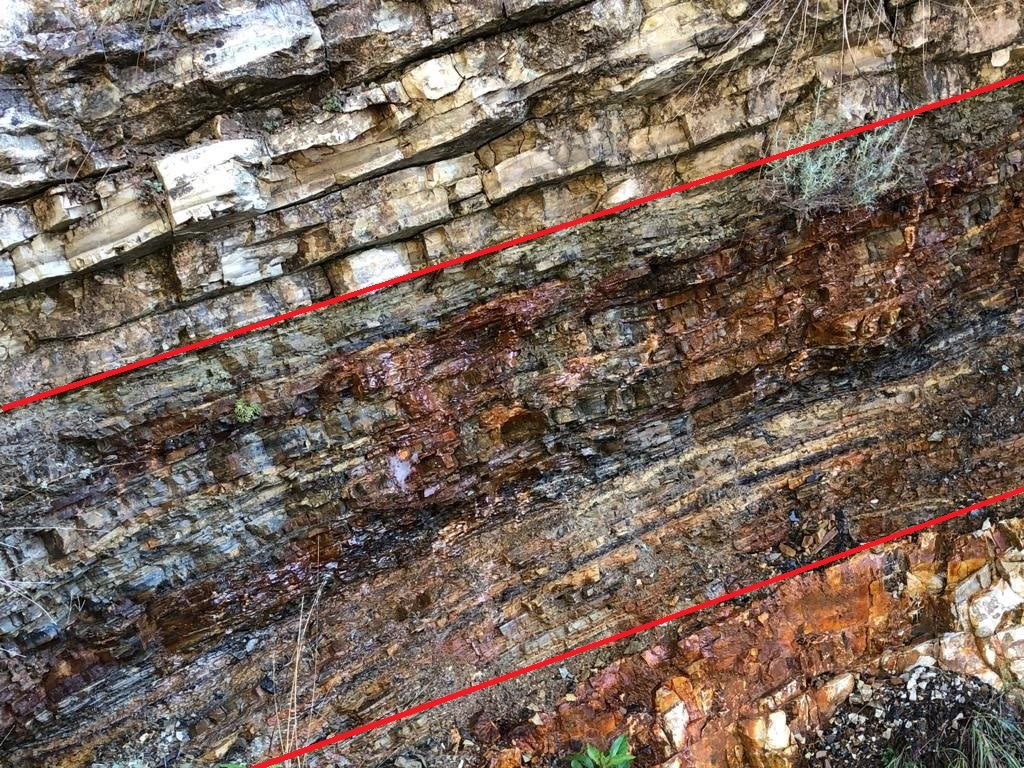
\includegraphics[width=0.66\linewidth]{images/book4/b2-19-bonarelli-level.jpg}
\par\smallskip{\small बोनारेल्ली स्तर, OAE~2 का गहरा शेल, हल्के चूना-पत्थरों के बीच; फ़ोटोग्राफ़र द्वारा
खींची गई लाल रेखाएँ उसका आधार और शीर्ष चिह्नित करती हैं। (Picenus, CC~BY-SA~4.0, विकिमीडिया
कॉमन्स के माध्यम से।)}
\end{omfigure}
% ledger: rigo24:oaes

\begin{inthefield}[एक अनॉक्सी घटना का लॉग]
पेलैजिक चूना-पत्थरों के किसी खंड में OAE का अध्ययन करने वाली भूविज्ञानी उसे परत-दर-परत लॉग करती है: मोटाई,
रंग, पटलन, बिल या उनका अभाव, पायराइट की गुलिकाएँ। वह गहरे अंतराल के आर-पार और उससे बहुत आगे तक
पास-पास, नियमित अंतरालों पर नमूने लेती है, कार्बनिक कार्बन की मात्रा के लिए और
कार्बनिक पदार्थ तथा कार्बोनेट के कार्बन समस्थानिकों के लिए; समस्थानिकों का विचलन, चट्टान के
रंग से अधिक, घटना को एक द्रोणी से दूसरी तक सहसंबद्ध करता है। क्योंकि सबसे गहरा
शेल अलग-अलग द्रोणियों में अलग-अलग स्तरों पर दिख सकता है, काला शेल नहीं बल्कि समस्थानिक-वक्र
समय-रेखा माना जाता है।
\end{inthefield}
% ledger: rigo24:oaes, wt24:oae2

\subsection*{चिक्सुलूब}

क्रिटेशियस के अंत का कारण बाहर से आया। पुस्तक 3 ने बताया था कि सीमा की मिट्टी के इरिडियम ने
एक आघात तक कैसे पहुँचाया, और आर्गन काल-निर्धारण ने सीमा को चिक्सुलूब क्रेटर से कैसे जोड़ा।
संरचना लगभग \qty{200}{km} चौड़ी और \qty{66}{Ma} पुरानी है; उसकी
गर्म चट्टानों ने उसके बाद कम से कम आठ मिलियन वर्षों तक परिसंचारी जल को ऊष्मा दी। उसकी उपसतही
असममिति के मॉडल एक ऐसे आघातकारी पिंड की ओर संकेत करते हैं जो उत्तर-पूर्व से क्षैतिज से 45 से \ang{60} पर आया,
पृथ्वी के पलायन वेग, \qty{11.2}{km.s^{-1}}, से कम नहीं, और अधिक संभवतः लगभग
\qty{20}{km.s^{-1}} पर। डेक्कन ट्रैप्स उसी समय फूट रहे थे, आघात से पहले और बाद में;
2010 में साक्ष्यों की एक समीक्षा ने निष्कर्ष निकाला कि आघात ने विलोपन को आरंभ किया।
% ledger: pickersgill26:chicxulub, collins20:impact, renne:kpg, alvarez:iridium, schulte:kpg, cr03:deccan

\begin{dated}{2026}
इस अध्याय की आयुएँ अंतर्राष्ट्रीय कालस्तरिक चार्ट के जून 2026 संस्करण की हैं,
जैसा इस पूरी शृंखला में प्रयुक्त है; समुद्र-स्तर के अभिलेख अपनी फ़ाइलों के 2012 के समय-मापक्रम
पर हैं, और विलोपन-आयुएँ काइहो (2022) की हैं। नई तिथियाँ आने पर चार्ट संशोधित होता है:
किसी सीमा-आयु को उद्धृत करने से पहले वर्तमान संस्करण देख लीजिए।
\end{dated}
% ledger: ics:base.Phanerozoic, data:b4-sealevel, kaiho22:table

\section*{अभ्यास}\label{sec:b2:phanerozoic-earth:exercises}

अभ्यासों के आँकड़े, अन्यथा न कहा जाए तो: अक्षांश के प्रति अंश \qty{111.2}{km}; महासागर-तल
की गहराई $d(t) = 2500 + 350\sqrt t$ (\unit{m}, $t$ \unit{Myr} में); महासागर का क्षेत्रफल
\qty{362}{\mega km^2}; महासागर-तल का क्षेत्रफल \qty{293}{\mega km^2}; प्रावार का घनत्व
\qty{3300}{kg.m^{-3}}; समुद्री जल \qty{1025}{kg.m^{-3}}; वायुमंडल का द्रव्यमान
\qty{5.1e18}{kg}, वायु और कार्बन डाइऑक्साइड के मोलर द्रव्यमान \qty{28.97}{g.mol^{-1}} और
\qty{44.01}{g.mol^{-1}}।
% ledger: earth:Rmean, ps77:depth-age, charette:ocean-volume, data:b4-ridge, katz03:thermo, noaa:seawater-1025, earth:Matm, earth:Mmol, ciaaw:abridged-2024

\begin{exercise}[$\star$]\label{exo:b2:phanerozoic-earth:1}
मानचित्रों के मॉडल में केप टाउन \ang{61.9}~S पर था, \qty{300}{Ma} पहले, और न्यूयॉर्क
\ang{3.6}~S पर; आज वे \ang{33.9}~S और \ang{40.7}~N पर हैं। (क)~चारों नगरों में से कौन भूमध्य रेखा के
\ang{30} के भीतर था, \qty{300}{Ma} पहले (पेरिस \ang{5.1}~N पर, सिडनी
\ang{59.5}~S पर)? (ख)~तब से केप टाउन और न्यूयॉर्क में से हर एक कितने किलोमीटर उत्तर खिसका है?
(ग)~किन माध्य दरों से, सेंटीमीटर प्रति वर्ष में?
\end{exercise}
% ledger: data:b4-palaeopos, geonames4:cities

\begin{exercise}[$\star$]\label{exo:b2:phanerozoic-earth:2}
बड़े पाँच 444, 372, 251.9, 201.4 और \qty{66}{Ma} पर पड़े। (क)~क्रमिक संकटों के बीच के
अंतराल और उनका माध्य ज्ञात कीजिए। (ख)~बृहत आग्नेय प्रांतों की माध्य आयुओं का उपयोग करके ---
एमेइशान 259, साइबेरियाई 250, CAMP 201, कारू--फ़ेरार 183, डेक्कन \qty{65.5}{Ma} --- पाँचों में से
कौन-से किसी प्रांत के \qty{2}{Myr} के भीतर पड़ते हैं? (ग)~क्या एक माध्य अंतराल संकटों को आवर्ती बनाता है?
\end{exercise}
% ledger: kaiho22:table, cr03:table

\begin{exercise}[$\star$]\label{exo:b2:phanerozoic-earth:3}
मॉन्यूमेंट रॉक्स की खड़िया लगभग \qty{0.036}{mm} प्रति वर्ष की दर से जमी। (क)~उसके
\qty{91}{m} में कितना समय लगा? (ख)~आज समुद्र, \qty{3.7}{mm} प्रति
वर्ष पर, कितने गुना तेज़ी से उठता है? (ग)~एक समुद्र-तल कीचड़ में दबे बिना अवसाद की इतनी धीमी वर्षा कैसे एकत्र कर सकता है?
\end{exercise}
% ledger: kgs:monument-rocks, ipcc:sea-level-obs

\begin{exercise}[$\star$]\label{exo:b2:phanerozoic-earth:4}
एक खड़ी चट्टान में, नीचे से ऊपर: जड़ों वाला नदी-बलुआ पत्थर, सीपियों वाली समुद्र-तट की बालू, तट से दूर की धूसर
कीचड़, खड़िया; फिर खड़िया के ऊपर फिर से समुद्र-तट की बालू। (क)~खंड कहाँ एक
\omterm{def:b2:phanerozoic-earth:transgression}{समुद्री ट्रांसग्रेशन} दर्ज करता है, और कहाँ एक रिग्रेशन? (ख)~क्या ट्रांसग्रेशन सिद्ध करता है कि वैश्विक
समुद्र-स्तर उठा? (ग)~उसे अधिक विश्वसनीय क्या बनाएगा?
\end{exercise}

\begin{exercise}[$\star\star$]\label{exo:b2:phanerozoic-earth:5}
हक़ और अन्य के दीर्घकालिक वक्र पर समुद्र-स्तर आज से \qty{233}{m} ऊपर था,
\qty{97}{Ma} पर। (क)~तब से गिरावट की माध्य दर क्या है, मीटर प्रति मिलियन वर्ष में और
माइक्रोमीटर प्रति वर्ष में? (ख)~आज की \qty{3.7}{mm} प्रति वर्ष की वृद्धि से तुलना कीजिए। (ग)~बैकस्ट्रिप किया
न्यू जर्सी वक्र उसी समय लगभग \qty{70}{m} देता है। आयाम के लिए आप किस पर भरोसा करेंगे,
और क्यों?
\end{exercise}
% ledger: data:b4-sealevel, ipcc:sea-level-obs, miller05:abstract, miller20:epr

\begin{exercise}[$\star\star$]\label{exo:b2:phanerozoic-earth:6}
CAMP का एक अकेला स्पंद, लगभग \qty{e5}{km^3} बेसाल्ट, घनत्व \qty{2900}{kg.m^{-3}},
लगभग 500 वर्षों में फूटा। (क)~द्रव्यमान से \qty{0.75}{\percent} कार्बन डाइऑक्साइड के साथ, उसने कितनी
छोड़ी, किलोग्राम में और मोल में? (ख)~1750 के \qty{278}{ppm} पर वायु में कितना
कार्बन डाइऑक्साइड द्रव्यमान था? (ग)~तुलना कीजिए। (घ)~पूरा प्रांत,
\qty{e5}{Gt}, ऐसे कितने वायुमंडल दे पाता?
\end{exercise}
% ledger: capriolo20:camp-co2, ipcc:erf-2xco2, earth:Matm, earth:Mmol, ciaaw:abridged-2024

\begin{exercise}[$\star\star$]\label{exo:b2:phanerozoic-earth:7}
चिक्सुलूब आघातकारी पिंड को \qty{10}{km} व्यास का, घनत्व
\qty{2630}{kg.m^{-3}} का एक गोला मानिए। (क)~उसका द्रव्यमान ज्ञात कीजिए। (ख)~न्यूनतम संभव
चाल, \qty{11.2}{km.s^{-1}}, पर और \qty{20}{km.s^{-1}} पर उसकी गतिज ऊर्जा ज्ञात कीजिए। (ग)~पृथ्वी अपनी सतह से
\qty{47}{TW} आंतरिक ऊष्मा खोती है। हर ऊर्जा उस क्षति के कितने वर्षों के बराबर है?
\end{exercise}
% ledger: alvarez:iridium, collins20:impact, b2dd10:half-space

\begin{exercise}[$\star\star$]\label{exo:b2:phanerozoic-earth:8}
(क)~उन लक्षणों की सूची बनाइए जिनसे एक काला शेल \omterm{def:b2:phanerozoic-earth:oae}{महासागरीय अनॉक्सी घटना} दर्ज करता है। (ख)~हर
घटना को लगभग समान आयु के एक प्रांत से जोड़िए: आरंभिक टोआर्सियन, \qty{183}{Ma}; OAE~1a,
\qty{120}{Ma}; दिया है कारू--फ़ेरार \qty{183}{Ma} पर और ओंटोंग जावा \qty{122}{Ma} पर। (ग)~आयुओं का
संयोग यह सिद्ध करने के लिए पर्याप्त क्यों नहीं कि किसी प्रांत ने कोई घटना उत्पन्न की?
\end{exercise}
% ledger: rigo24:oaes, cr03:table

\begin{exercise}[$\star\star$]\label{exo:b2:phanerozoic-earth:9}
मॉडल में पेरिस \ang{60.9}~S पर था, \qty{500}{Ma} पहले, और \ang{5.1}~N पर, \qty{300}{Ma} पहले।
(क)~उसका उत्तरमुखी विस्थापन अंशों और किलोमीटरों में ज्ञात कीजिए, और माध्य दर
सेंटीमीटर प्रति वर्ष में। (ख)~\qty{300}{Ma} से की दर से तुलना कीजिए
(\cref{ex:b2:phanerozoic-earth:paris})। (ग)~यह दर न्यूनतम क्यों है?
\end{exercise}
% ledger: data:b4-palaeopos

\begin{exercise}[$\star\star\star$]\label{exo:b2:phanerozoic-earth:10}
मान लीजिए इसके बजाय तल का क्षेत्रफल आयु के साथ रैखिक रूप से घटता है, आयु 0 पर अधिकतम से आयु $T$ पर
शून्य तक। (क)~दिखाइए कि माध्य आयु $T/3$ है और $\sqrt t$ का माध्य
$\tfrac{8}{15}\sqrt T$ है। (ख)~\qty{64.2}{Myr} की माध्य आयु के साथ $T$ और माध्य गहराई ज्ञात कीजिए। (ग)~प्रसरण-दर
दुगुनी होने पर माध्य गहराई की गिरावट ज्ञात कीजिए, और समान मॉडल के
\qty{774}{m} से तुलना कीजिए। (घ)~दिखाइए कि दोनों मॉडलों में गिरावट $0.93\,c\sqrt{\bar
t}\,(1 - f^{-1/2})$ के निकट है, जहाँ $\bar t$ माध्य आयु है।
\end{exercise}

\begin{exercise}[$\star\star\star$]\label{exo:b2:phanerozoic-earth:11}
(क)~\cref{prop:b2:phanerozoic-earth:ridge} से दिखाइए कि $\Delta s(f) = \Delta s(2)\,(1 -
f^{-1/2})/(1 - 2^{-1/2})$। (ख)~$\Delta s(2) = \qty{432}{m}$ के साथ $f$ का वह परास ज्ञात कीजिए जो
क्रिटेशियस शिखर, 50 से \qty{150}{m}, देता है। (ग)~आज की 0.8 तक धीमी हुई प्रसरण-दर
क्या करती? (घ)~कटकों द्वारा तय दीर्घकालिक समुद्र-स्तर एक धीमा संकेत क्यों है, दर का परिवर्तन
कुछ भी हो?
\end{exercise}
% ledger: data:b4-ridge, miller05:abstract

\begin{exercise}[$\star\star\star$]\label{exo:b2:phanerozoic-earth:12}
मान लीजिए प्रजातियाँ एक स्थिर दर से लुप्त होती हैं, ताकि किसी समूह का जो अंश समय $t$ तक जीवित रहता है
वह $2^{-t/m}$ है, जहाँ प्रजातियों की माध्यिका आयु $m = \qty{2}{Myr}$ है। (क)~\qty{7.4}{Myr} के बाद, जो 1982 के विश्लेषण की माध्य चरण-लंबाई है,
किसी समूह का कितना अंश जा चुका होता है? (ख)~पृष्ठभूमि विलोपन को
प्रजातियों का \qty{81}{\percent} हटाने में कितना समय लगता? (ग)~पर्मियन-अंत संकट लगभग
\qty{60}{kyr} चला। वह कितना तेज़ था? (घ)~मोटा काल-विभेदन सामूहिक विलोपन
और पृष्ठभूमि विलोपन के अंतर को धुंधला क्यों कर देता है?
\end{exercise}
% ledger: marshall23:resolution, stanley16:permian, burgess:end-permian

\begin{problem}[{सप्ताहांत समस्या --- जब कटक तेज़ थे}]\label{pb:b2:phanerozoic-earth:1}
यह समस्या पूछती है कि यदि कटक दुगुनी तेज़ी से फैलते तो समुद्र कितना उठता, और वह कितनी भूमि
डुबोता। अभ्यासों के आँकड़े लीजिए; महासागर-तल की माध्य आयु
\qty{64.2}{Myr} है, कटकों की कुल लंबाई \qty{65000}{km} है, आज का महासागर
\qty{1.33e9}{km^3} रखता है, और भूमि \qty{148}{\mega km^2} ढकती है। तालिका आज की भूमि का वह प्रतिशत देती है
जो समुद्र-स्तर से $h$ से कम ऊपर है, एक-अंश ETOPO1 ग्रिड से।
\begin{center}
\small
\begin{tabular}{lcccccc}
\hline
$h$ (\unit{m}) & 0 & 100 & 200 & 300 & 400 & 500 \\
$h$ से नीचे भूमि (\unit{\percent}) & 0 & 14.9 & 28.2 & 38.7 & 48.1 & 55.8 \\
\hline
\end{tabular}
\end{center}
\cref{prop:b2:phanerozoic-earth:ridge} की तरह मान लीजिए कि 0 और उस
आयु $\tau$ के बीच, जिस पर तल क्षेपित होता है, तल की हर आयु समान क्षेत्रफल घेरती है।

\noindent\textbf{भाग I --- आज का महासागर-तल।}
\begin{enumerate}
  \item 0, 25, 64.2 और \qty{100}{Myr} की आयुओं पर तल की गहराई ज्ञात कीजिए।
  \item माध्य आयु से $\tau$ ज्ञात कीजिए, और सबसे पुराने तल की गहराई।
  \item माध्य पूर्ण प्रसरण-दर $u = A_{\text{f}}/(L\tau)$ ज्ञात कीजिए, किलोमीटर प्रति मिलियन
        वर्ष में और मिलीमीटर प्रति वर्ष में। क्या यह धीमी, मध्यम या तेज़ दर है?
  \item दिखाइए कि तल की माध्य गहराई $2500 + \tfrac23 \times 350\sqrt\tau$ है, और
        उसकी गणना कीजिए।
  \item दिनांकित तल की मापी गई माध्य गहराई \qty{4265}{m} है। दो कारण दीजिए कि
        मॉडल अधिक गहरा क्यों है।
  \item मॉडल में तल के ऊपर कितना जल-आयतन होता? पूरे महासागर के आयतन से
        तुलना कीजिए।
\end{enumerate}

\noindent\textbf{भाग II --- अनुप्रस्थ काट में एक कटक।}
\begin{enumerate}[resume]
  \item अर्ध प्रसरण-दर $v$, निकटतम \qty{0.1}{km.Myr^{-1}} तक, और कटक के हर ओर
        तल की चौड़ाई ज्ञात कीजिए।
  \item अक्ष से \qty{1000}{km} दूर तल कितना गहरा है?
  \item दिखाइए कि सबसे पुराने तल की गहराई से ऊपर कटक की अनुप्रस्थ काट, दोनों
        पार्श्व गिनकर, क्षेत्रफल $\tfrac23 v c\,\tau^{3/2}$ रखती है, और उसकी गणना
        वर्ग किलोमीटर में कीजिए।
  \item उस गहराई से ऊपर पूरे कटक-तंत्र का आयतन ज्ञात कीजिए।
  \item यह महासागर के आयतन का कितना अंश है?
  \item तेज़ी से फैलता कटक औसतन अधिक ऊँचा क्यों खड़ा रहता है?
\end{enumerate}

\noindent\textbf{भाग III --- दुगुनी तेज़ी।}
\begin{enumerate}[resume]
  \item प्रसरण-दर उसी तल-क्षेत्रफल और कटक-लंबाई के साथ दुगुनी होती है। नया $\tau$
        और नई माध्य गहराई ज्ञात कीजिए।
  \item माध्य गहराई कितनी घटती है?
  \item तल द्रोणियों से कितना जल-आयतन बाहर धकेलता है?
  \item आज के महासागर पर फैलाने पर वह समुद्र को कितना उठाता?
  \item वृद्धि $\Delta s$ ज्ञात करने के लिए अतिरिक्त जल के नीचे तल के धँसने को सम्मिलित कीजिए।
  \item दीर्घकालिक क्रिटेशियस शिखर लगभग \qty{100}{m} था। प्रसरण-दर की कितनी वृद्धि
        वह देती?
\end{enumerate}

\noindent\textbf{भाग IV --- भूमि पर समुद्र।}
\begin{enumerate}[resume]
  \item \qty{100}{m} की वृद्धि कितना भूमि-क्षेत्र डुबोती?
  \item तालिका में अंतर्वेशन से, \qty{432}{m} की वृद्धि कितना क्षेत्र डुबोती?
  \item भूमि पर फैलने के बाद समुद्र को \qty{432}{m} से कम क्यों उठना होगा?
  \item \qty{100}{m} के चरणों में \qty{400}{m} तक समुद्र उठाने के लिए आवश्यक आयतन ज्ञात कीजिए,
        हर चरण पर डूबे क्षेत्रफल का औसत लेकर (\cref{prop:b2:phanerozoic-earth:flooding})।
        रखा जाने वाला आयतन $\qty{0.432}{km} \times \qty{362}{\mega km^2}$ है। समुद्र
        कहाँ रुकता है?
  \item तब वह आज की भूमि का कितना प्रतिशत ढकता है?
  \item सारांश: इस मॉडल में प्रसरण-दर दुगुनी करने से समुद्र कितना उठता?
\end{enumerate}
\end{problem}
% ledger: ps77:depth-age, seton:mean-age, seton:rate-classes, noaa:ridge, charette:ocean-volume, data:b4-ridge, data:b4-floor-depth, katz03:thermo, noaa:seawater-1025, data:b4-hyps, miller05:abstract
